\section{Algoritmi sequenziali e richiami}
Prima di entrare nel vivo del corso è necessario richiamare alcuni concetti e dinamiche visti nel corso di architetture degli elaboratori. Anzitutto, un \textbf{algoritmo sequenziale} è un insieme finito di istruzioni elementari, eseguibili in modo deterministico da una macchina astratta. Tale macchina rappresenta un modello teorico di calcolo e possiede le seguenti caratteristiche: \begin{itemize}
	\item \textbf{Il calcolo è discreto}: L’esecuzione avviene come sequenza di passi elementari, ciascuno dei quali richiede tempo finito.
	\item \textbf{Il comportamento è deterministico}: A parità di stato iniziale e input, l’evoluzione del calcolo è univocamente determinata.
	\item \textbf{La memoria è idealmente illimitata}.
	\item \textbf{Ogni dato manipolato ha dimensione finita}, ma non esiste un limite prefissato alla quantità totale di memoria utilizzabile.
\end{itemize}
\noindent I suddetti algoritmi sono espressi in un linguaggio di programmazione, al quale è associata una macchina astratta capace di eseguire i programmi scritti in tale linguaggio. In particolare, descriviamo tali macchine tramite tre componenti fondamentali: \begin{itemize}
	\item \textbf{Memoria}: Insieme idealmente infinito di celle per memorizzazione dati, tale che: \begin{itemize}
		\item Ogni cella è identificata da un indirizzo univoco.
		\item L’associazione tra celle e indirizzi è biunivoca.
		\item Ogni cella può contenere un valore, ed ogni possibile associazione celle-valori memorizzati fornisce una configurazione particolare della memoria.
	\end{itemize}
	\item \textbf{Ambiente}: Associazione tra un insieme finito di identificatori (variabili) e indirizzi di memoria. Consente di collegare i nomi simbolici utilizzati nel programma alle effettive locazioni di memoria.
	\item \textbf{Interprete}: Meccanismo per l'esecuzione delle istruzioni tramite il ciclo fetch-code-execute.
\end{itemize}

%

\section{Organizzazione di un sistema elaborativo}
Il \textbf{sistema operativo} è lo strato di software che gestisce le risorse hardware di un elaboratore e fornisce servizi a utenti e programmi applicativi. Svolge il ruolo di intermediario tra hardware e utente, con gli obiettivi principali di rendere conveniente l'uso del sistema per l'utente e garantire un utilizzo efficiente delle risorse hardware. Si tratta di una delle quattro componenti dei sistemi di calcolo moderni, insieme all'hardware, gli applicativi e gli utenti.
\begin{figure}[h]
	\centering
	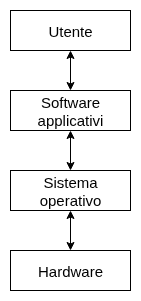
\includegraphics[width=0.2\textwidth]{Images/AbstractComponents.png}		
	\caption{Componenti astratte di un elaboratore moderno}
	\label{fig:AbstractComponents}
\end{figure}

\noindent La componente centrale del sistema operativo è il \textbf{kernel}, un processo eseguito in modalità privilegiata costantemente in background per fornire meccanismi fondamentali per la gestione degli altri processi e delle risorse. Gestisce direttamente, tra l'altro, CPU, memoria e periferiche I/O.\par
I programmi che forniscono funzionalità di base non facenti parte del kernel sono detti \textbf{programmi di sistema} e sono per esempio la shell o i compilatori, mentre gli altri programmi sono detti \textbf{applicativi}. Molti sistemi moderni includono inoltre uno strato software aggiuntivo detto \textbf{middleware}, che fornisce servizi di alto livello come database, sistemi grafici o infrastrutture distribuite.
\begin{figure}[h]
	\centering
	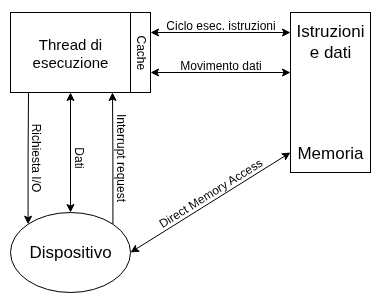
\includegraphics[width=0.7\linewidth]{Images/ModernPCDynamic.png}
	\caption{Funzionamento di un elaboratore moderno}
	\label{fig:ModernPCDynamic}
\end{figure}
\noindent All’accensione del calcolatore, l’esecuzione inizia da un programma \textbf{bootloader} residente nel firmware (BIOS o UEFI), il cui compito è inizializzare l’hardware e caricare in memoria un programma di \textbf{bootstrap}. Il bootloader provvede quindi a caricare il kernel del sistema operativo in memoria e a trasferirgli il controllo.\par
Inizializzato, il kernel configura le strutture dati fondamentali, inizializza i dispositivi e avvia i primi processi di sistema. Terminata questa fase, il sistema entra in una modalità di esecuzione guidata dagli eventi. Il controllo del processore passa tra processi e kernel in risposta a interrupt hardware, eccezioni oppure trap, quindi richieste di servizio da parte dei programmi utente.

%

\section{Attività del sistema operativo}
Fra le principali caratteristiche dei sistemi operativi moderni vi è inoltre la \textbf{multiprogrammazione}. Un singolo programma non utilizza costantemente la CPU: durante le operazioni di input/output o in attesa di eventi, il processore rimarrebbe inattivo. Con questo meccanismo si aumenta il suo utilizzo mantenendo in memoria più programmi contemporaneamente.\par
Il sistema operativo salva temporaneamente in memoria centrale alcuni programmi, in questo caso detti \textbf{processi}, e ne sceglie uno per l'esecuzione. Quando il processo scelto deve attendere un evento, la CPU viene assegnata ad un altro processo pronto. Dandole costantemente nuovi compiti quando sono disponibili si riduce il sul tempo di inattività.
\begin{figure}[h]
	\centering
	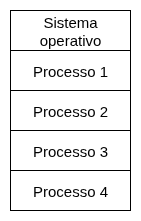
\includegraphics[width=0.2\linewidth]{Images/MemConf_multiprogrammedOS.png}
	\caption{Configurazione di memoria per sistemi multiprogrammati}
	\label{fig:MultOS}
\end{figure}

\noindent Un'estensione logica della multiprogrammazione è il \textbf{multitasking}, detto anche time sharing. Si tratta di un modello nel quale la CPU è assegnata ai processi per intervalli di tempo molto piccoli e limitati, detti \textbf{quanti}. Il cambio tra i processi è gestito dallo \textbf{scheduler} del processore, ed è effettuato ad una frequenza tale da creare l'impressione di un'esecuzione simultanea, garantendo buoni tempi di risposta.\par
Poiché le risorse hardware sono condivise, esistono alcuni meccanismi per garantire un'efficiente esecuzione dei programmi, come anche la protezione del sistema operativo. Il primo è dato dalla \textbf{memoria virtuale}, la quale consente di eseguire processi non completamente salvati in memoria fisica tramite una sua astrazione. Il secondo riguarda la \textbf{modalità duale di funzionamento}, che garantisce protezione tra sistema operativo e programmi utente; in particolare distingue tramite un \textbf{bit di modalità} le: \begin{itemize}
	\item \textbf{Modalità kernel 0}: Per eseguire istruzioni privilegiate.
	\item \textbf{Modalità utente 1}: Per eseguire istruzioni accessibili all'utente.
\end{itemize}
\noindent Siccome l'accesso alle istruzioni critiche è precluso agli utenti, quando un programma necessita di un servizio del sistema operativo, invoca una \textbf{system call}. Questa genera una \textbf{trap}, vista dal sistema come interruzione, e l'hardware passerà in modalità kernel. Il controllo passa ora a una routine del sistema operativo, individuata tramite un vettore con i valori relativi alle trap. Si esegue ora il servizio richiesto e il controllo ritorna al programma utente in user mode.\par
Se durante l'esecuzione si verifica una condizione anomala, come per esempio un accesso a memoria non valida o divisione per zero, l’hardware genera un’\textbf{eccezione}. In tal caso il controllo passa al sistema operativo, che può terminare il processo, segnalare l'errore ed eseguire eventuali azioni correttive. In alcuni sistemi, se la funzione è presente, possono essere generati dei file testuali detti \textbf{memory dump} per analisi successive.\par
Un ulteriore meccanismo di protezione è rappresentato dal \textbf{timer} hardware; un contatore che al raggiungimento dello zero genera un interrupt. Si tratta di una componente essenziale per in primo luogo implementare il time sharing, ma anche per impedire che un processo monopolizzi la CPU, garantendo che il controllo ritorni al sistema operativo entro un certo intervallo di tempo.

%

\section{Gestione delle risorse}
Per svolgere i propri compiti, un processo richiede alcune risorse, come memoria, file o tempo di CPU. Queste possono essergli assegnate alla sua nascita oppure in esecuzione, per poi essere rese al sistema operativo al termine del processo. In particolare diciamo che i programmi sono entità passive, mentre i processi sono attivi; questi ultimi si dividono in: \begin{itemize}
	\item \textbf{Single-threaded}: Contengono un solo thread di esecuzione, quindi un unico program counter.
	\item \textbf{Multi-threaded}: Contengono più fili di esecuzione, ciascuno con il proprio program counter e stack.
\end{itemize}
\noindent Tipicamente i sistemi attuano più processi concorrentemente; ciò ha luogo grazie ad un multiplexing della CPU tra \textbf{processi e thread}. Per quanto riguarda la loro \textbf{gestione}, i sistemi operativi sono responsabili della creazione e cancellazione dei processi utenti e di sistema, schedulazione di processi e thread sulle CPU, sospensione e ripristino dei processi ed infine della fornitura di meccanismi per la loro sincronizzazione e comunicazione.\par
Per eseguire un programma è necessario che almeno una parte delle sue istruzioni e relativi dati sia scritta nella memoria, in quanto è necessario accedervi per il loro funzionamento. Il programma genera così gli indirizzi logici, che verranno tradotti in indirizzi fisici dal sistema di \textbf{gestione della memoria}. In tal merito, il sistema operativo è responsabile di: \begin{itemize}
	\item Tenere traccia di quali zone di memoria sono usate e da chi.
	\item Assegnare e revocare lo spazio di memoria in base alle necessità.
	\item Decidere quali processi e dati debbano essere caricati in memoria centrale o trasferiti in quella di massa.
\end{itemize}
\noindent Il sistema operativo fornisce inoltre un'interfaccia logica uniforme per la memorizzazione delle informazioni, detta \textbf{file}. Si tratta di un'astrazione logica per la memorizzazione indipendente dal dispositivo fisico. Ogni file è organizzato in \textbf{directory}, permettendo di ottenere una struttura gerarchica, e possono prendere più forme: \textbf{libera}, come per i file testuali, oppure \textbf{strutturata}, come per gli mp3. Per quanto riguarda la \textbf{gestione dei file}, il sistema operativo è responsabile di: \begin{itemize}
	\item Creazione e cancellazione di file e directory.
	\item Fornitura delle funzioni fondamentali per la gestione di file e directory.
	\item Associazione dei file ai dispositivi di memoria secondaria.
	\item Creazione di backup dei file su dispositivi di memorizzazione non volatili.
\end{itemize}
\noindent Poiché i programmi utilizzano i dispositivi di memoria secondaria come dischi rigidi per memorizzare dati e programmi, è di fondamentale importanza che sia gestita correttamente e in modo efficiente. Per la \textbf{memoria di massa}, infatti, il sistema operativo \textbf{gestisce}: \begin{itemize}
	\item Montare e smontare (mounting, unmounting) le unità di memoria.
	\item Assegnazione dello spazio e gestione dello spazio libero.
	\item Scheduling del disco.
	\item Partizionamento.
	\item Protezione.
\end{itemize}
\noindent Come già detto, più utenti possono usare uno stesso calcolatore ed è quindi necessario gestire l'accesso ai dati mediante apposite regole. Ciò avviene con la \textbf{protezione}: meccanismi di controllo dell'accesso alle risorse del PC da parte di processi o utenti. Ci sono varie strategie per attuarla, ma tutte devono fornire le specifiche dei controlli e gli strumenti utilizzati. Un altro concetto molto importante, a causa del costante incremento di attacchi informatici, è la \textbf{sicurezza}: la difesa del sistema da attacchi volti al sistema operativo.\par
Questi due concetti presuppongono che si riesca a distinguere i propri utenti da quelli non autorizzati; generalmente ciò avviene grazie agli identificatori utente, che garantiscono loro unicità. Quando un utente o un gruppo si collega al sistema, infatti, è presente una fase di autenticazione per determinare l'ID corretto e associarlo al processo dell'utente. Se richiesto, è inoltre possibile cambiare l'ID effettivo tramite un comando, ottenendo accesso a comandi privilegiati.\newline

\noindent Come ultimo concetto presentiamo la \textbf{virtualizzazione}, una tecnica che permette di astrarre l'hardware di un singolo computer, quindi tutte le sue componenti, in diversi ambienti di esecuzione, creando l'illusione di avere più sistemi operativi attivi allo stesso momento su un solo calcolatore, i quali sono capaci di interagire l'uno con l'altro. Otteniamo questa dinamica con le \textbf{macchine virtuali}, che consentono agli utenti di cambiare agevolmente il sistema operativo del quale si ha necessità. Un concetto simile è quello dell'\textbf{emulazione}, ovvero la simulazione tramite software di un hardware diverso da quello del calcolatore; tecnica usata spesso quando il tipo di CPU della macchina è diverso da quello desiderato.